% chktex-file 44 32 36 38 18 11 8 26

\pagestyle{DS_FP}
%\NomPrenomNote{}

\bigskip

\exods{0}
%%% POLYNESIE 2025 - J1 - exo1

\emph{Cet exercice porte sur les graphes, les protocoles réseaux et la programmation orientée objet.}

\section*{PARTIE A}


    Le graphe suivant modélise un ensemble de routeurs ; les sommets sont les routeurs, les arêtes les liaisons entre ceux-ci.

\begin{figure}[!h]
\begin{center}
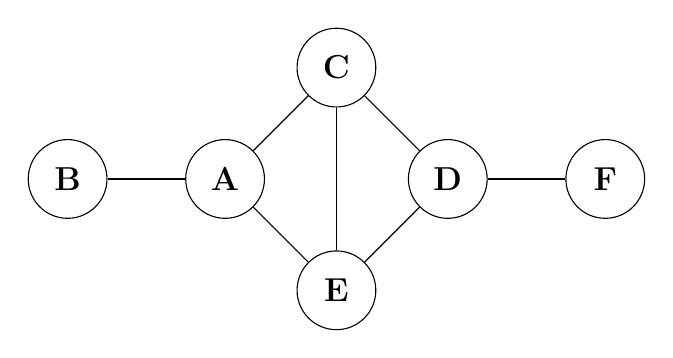
\begin{tikzpicture}[
    node distance={2cm}, 
    main/.style = {draw, circle, minimum size=1cm, font=\large\bfseries}
] 

    % Définition des nœuds (Nodes)
    \node[main] (B) {B};
    \node[main] (A) [right of=B] {A};
    \node[main] (C) [above right of=A] {C};
    \node[main] (E) [below right of=A] {E};
    \node[main] (D) [below right of=C] {D};
    \node[main] (F) [right of=D] {F};

    % Tracé des arêtes (Edges)
    \draw (B) -- (A);
    \draw (A) -- (C);
    \draw (A) -- (E);
    \draw (C) -- (E);
    \draw (C) -- (D);
    \draw (E) -- (D);
    \draw (D) -- (F);

\end{tikzpicture}
\end{center}
\caption{Schéma des routeurs et des liaisons}\label{reseau_exo1}
\end{figure}

On désire parcourir ce graphe en largeur depuis le sommet A. On considère que les sommets sont explorés dans l'ordre alphabétique.


\begin{enumerate}[series=monDS]
    \item Donner l'ordre de parcours des sommets du graphe.\hfill 

\end{enumerate}

Voici un résumé sommaire du fonctionnement du protocole RIP permettant à chaque routeur d’un réseau de taille modérée d’établir sa table de routage :\par


\textbf{Règle a (règle d’initialisation).} Chaque routeur initialise sa table en y ajoutant ses voisins directs. Ils sont accessibles en un saut, sans passer par aucun routeur intermédiaire.\par
\textbf{Règle b (règle de transmission/réception).} À intervalles de temps réguliers chaque routeur envoie sa table de routage à ses voisins.\par 
\textbf{Règle c (règle de mise à jour).} Lorsqu’un routeur reçoit les informations d’un routeur voisin, trois cas peuvent survenir :

\begin{itemize}
    \item une route vers un nouveau routeur lui est présentée : il l’ajoute à sa table de routage ;
    \item une route vers un routeur déjà connu lui est présentée, plus longue en nombre de sauts que celle inscrite dans sa table : elle est ignorée ;
    \item une route vers un routeur déjà connu lui est présentée, mais strictement plus courte en nombre de sauts que la précédente : l’ancienne est remplacée par celle-ci.

\end{itemize}

La réception par chaque routeur des tables de tous ses voisins et la mise à jour de sa table de routage en conséquence constitue une itération du protocole. Au bout d’un petit nombre de ces itérations, plus aucune table de routage ne varie, on dit que le processus est stabilisé.
\par 
Pour tout cet exercice, on n’envisagera pas les cas problématiques dans lesquels une liaison est coupée ou un routeur tombe en panne.

\par 
\begin{minipage}{0.48\linewidth}
    On considère des routeurs A, B, C, D, E et F connectés comme indiqué sur le graphe de la figure \ref{reseau_exo1}.
\medskip 
Voici la table de routage de A à l’initialisation du protocole RIP :

\end{minipage}\hfill{}
\begin{minipage}{0.52\linewidth}
    \centering
    \renewcommand{\arraystretch}{1.5} % Augmente l'espacement pour plus de lisibilité
    \begin{tabular}{|c|c|c|}
        \hline
        \multicolumn{3}{|c|}{\textbf{Table de routage de A}} \\
        \hline
        \textbf{routeur} & \textbf{nombre de sauts} & \textbf{prochain routeur} \\
        \hline
        B & 1 & -- \\
        \hline
        C & 1 & -- \\
        \hline
        E & 1 & -- \\
        \hline
    \end{tabular}
\end{minipage}



\begin{enumerate}[series=monDS, resume]
    \item Donner la table de routage de F à l’initialisation du protocole RIP.

    \medskip

    \item Donner la table de routage de A après une première itération de RIP (deux réponses sont possibles).
    
    \medskip
    \item Donner le numéro de l’itération de RIP à partir duquel les tables des routeurs du réseau ne varient plus. \hfill 
\end{enumerate}

\medskip

On suppose dans la question suivante que les routeurs E et F sont reliés.

\begin{enumerate}[series=monDS, resume]
    \item Donner la nouvelle table de routage de A après stabilisation de RIP (deux réponses sont possibles).

\end{enumerate}

\medskip

\section*{PARTIE B}

\medskip

Pour simuler la situation précédente et les tables de routage, on modélise le fonctionnement d’un routeur par la classe \verb|Routeur|. Chaque instance \verb|r| de la classe \verb|Routeur| possède quatre attributs.

\begin{itemize}
    \item \verb|nom| : une chaine de caractères qui identifie le routeur.
    \item \verb|voisins| : une liste d’objets de type Routeur. Il s’agit de routeurs qui sont directement connectés au routeur r.
    \item \verb|nb_sauts| : un dictionnaire qui associe à chaque routeur accessible depuis \verb|r| le nombre de sauts nécessaires pour l’atteindre depuis \verb|r|.
    \item \verb|prochain| : un dictionnaire qui associe à chaque routeur \verb|r_accessible|, accessible depuis \verb|r|, le premier routeur sur un chemin qui mène à \verb|r_accessible|, en \verb|n| sauts, où \verb|n| est la valeur associée à \verb|r_accessible| dans \verb|nb_sauts|. S’il y a un unique saut de \verb|r| à \verb|r_accessible|, alors la valeur associée au routeur \verb|r_accessible| est \verb|None|.
\end{itemize}

Initialement, tous les routeurs sont déconnectés : l’attribut \verb|voisins| est initialisé avec la liste vide, et les attributs \verb|nb_sauts| et \verb|prochain| avec le dictionnaire vide.

\begin{CodePythontexAlt}[TaillePolice=\large, Largeur=1\linewidth,Centre,Lignes=true,PremLigne=1]{}
class Routeur: 
    def __init__(self, nom): 
        self.nom = nom
        self.voisins = []
        self.nb_sauts = {}
        self.prochain = {}
    \end{CodePythontexAlt}

Dans le programme principal, on crée les routeurs de la manière suivante :

\begin{CodePythontexAlt}[TaillePolice=\large, Largeur=1\linewidth,Centre,Lignes=true,PremLigne=1]{}
A = Routeur('A') 
B = Routeur('B') 
C = Routeur('C') 
D = Routeur('D') 
E = Routeur('E') 
F = Routeur('F')
    \end{CodePythontexAlt}

Ainsi que la liste des routeurs

\begin{CodePythontexAlt}[TaillePolice=\large, Largeur=1\linewidth,Centre,Lignes=true,PremLigne=1]{}
liste_routeurs = [A, B, C, D, E, F]
    \end{CodePythontexAlt}

    Afin de pouvoir relier les routeurs entre eux, on souhaite écrire une méthode \verb|relie|, de la classe \verb|Routeur|, dont on donne le code incomplet ci-dessous. Cette méthode prend en argument le routeur \verb|self| ainsi qu’un routeur \verb|autre| et met à jour si nécessaire les attributs \verb|voisins|, \verb|nb_sauts| et \verb|prochain| des routeurs \verb|self| et \verb|autre| afin d’indiquer la présence d’une connexion entre ces deux routeurs. Dans le cas où les routeurs sont déjà connectés, cette méthode ne fait rien.

    \begin{CodePythontexAlt}[TaillePolice=\large, Largeur=1\linewidth,Centre,Lignes=true,PremLigne=1]{}
def relie(self, autre): 
    if autre not in self.voisins: 
        self.voisins.append(...) 
        self.nb_sauts[autre] = ... 
        self.prochain[autre] = ... 
        if self not in autre.voisins: 
            autre.relie(...)
    \end{CodePythontexAlt}

    \begin{enumerate}[series=monDS, resume]
        \item Compléter le code de la méthode \verb|relie|.

\medskip

        \item Écrire la méthode \verb|relie_liste| de la classe \verb|Routeur| qui prend en paramètre une liste de routeurs \verb|lst| et qui relie le routeur \verb|self| à chacun des routeurs de la liste \verb|lst|.
        

    \end{enumerate}

    Par exemple, pour relier le routeur \verb|A| aux routeurs \verb|B|, \verb|C| et \verb|E|, on exécute l’instruction :

    \begin{CodePythontexAlt}[TaillePolice=\large, Largeur=1\linewidth,Centre,Lignes=true,PremLigne=1]{}

A.relie_liste([B, C, E]) 
# On n'appelle pas B.relie(A) car la liaison est déjà faite
    \end{CodePythontexAlt}

        \begin{enumerate}[series=monDS, resume]
\item Écrire les instructions manquantes pour relier les routeurs de manière à obtenir le graphe de la figure \ref{reseau_exo1}.



\end{enumerate}

D’après la règle c (règle de mise à jour) du protocole RIP, lorsqu’un routeur reçoit les informations d’un routeur voisin, il doit mettre à jour sa table de routage. On donne ci-dessous le code incomplet de la méthode \verb|met_a_jour_table| qui implémente la règle c du protocole RIP.

    \begin{CodePythontexAlt}[TaillePolice=\large, Largeur=1\linewidth,Centre,Lignes=true,PremLigne=1]{}
def met_a_jour_table(self, autre): 
    for r in autre.nb_sauts: 
        if r != self: 
            if (r not in self.nb_sauts or self.nb_sauts[r] > ...): 
                self.nb_sauts[r] = ... 
                self.prochain[r] = ...
\end{CodePythontexAlt}

\begin{enumerate}[series=monDS, resume]
    \item Compléter le code de la méthode \verb|met_a_jour_table| ci-dessus.
    
\medskip
    \item Écrire la méthode \verb|itere_rip| qui prend en paramètre le routeur \verb|self| et met à jour sa table de routage lorsqu’il reçoit la table de routage de chacun des routeurs présents dans la liste de ses voisins.

    \medskip
    \item Écrire une fonction qui prend en paramètre une liste de routeurs \verb|l_routeurs| et qui réalise une itération du protocole RIP pour tous les routeurs de \verb|l_routeurs|.


\end{enumerate}

Au bout de quelques itérations, le protocole RIP converge : plus aucune table de routage du réseau n’est modifiée. On aimerait pouvoir itérer le protocole dans le programme principal jusqu’à ce que ce soit le cas, à l’aide d’une boucle \verb|while|.\par

On suppose que la méthode \verb|met_a_jour_table| de la classe \verb|Routeur| a été modifiée de telle sorte qu’elle renvoie \verb|True| dans le cas où le routeur \verb|self| a procédé à une mise à jour de sa table de routage, et \verb|False| sinon.


\begin{enumerate}[series=monDS, resume]
    \item Écrire une version modifiée du code de la méthode \verb|itere_rip| de la classe \verb|Routeur| de telle sorte que celle-ci renvoie \verb|True| dans le cas où le routeur \verb|self| a procédé à une modification de sa table de routage au cours de lexécution de la méthode \verb|itere_rip|, et \verb|False| sinon.

\end{enumerate}

On donne ci-dessous le code du programme principal. On suppose que les instructions permettant de relier les routeurs ont été écrites à la suite et que la situation est celle décrite dans le graphe de la figure \ref{reseau_exo1}.

    \begin{CodePythontexAlt}[TaillePolice=\large, Largeur=1\linewidth,Centre,Lignes=true,PremLigne=1]{}
A = Routeur('A') 
B = Routeur('B') 
C = Routeur('C') 
D = Routeur('D') 
E = Routeur('E') 
F = Routeur('F') 
liste_routeurs = [A, B, C, D, E, F]
# instructions permettant de relier les routeurs
\end{CodePythontexAlt}

\begin{enumerate}[series=monDS, resume]
    \item Compléter le code du programme principal afin que celui-ci mette à jour les tables de routage des routeurs présents dans la liste \verb|liste_routeurs| jusqu’à ce qu’il ne soit plus nécessaire de faire des mises à jour des tables de routage.

    On ne demande pas de réécrire les instructions permettant de connecter les routeurs entre eux.

\end{enumerate}